\begin{activity}{Tower Hill Magnetics: Righting the Anomaly}

\section*{Purpose}

This case study applies the Fourier-domain magnetic processing ideas from the RTP demo to real aeromagnetic data from the Tower Hill Volcanic Complex in south-western Victoria, Australia. Unlike gravity, magnetic anomalies are inherently asymmetric -- their shape depends not just on source geometry but on the direction of the inducing field. Reduction to the pole (RTP) is a Fourier-domain phase correction that removes this asymmetry, but it is a fragile operation: powerful where it works, and prone to specific, predictable failure modes.

The activity progresses from a synthetic, idealized maar (where you know the true geometry) to the real Tower Hill data (where you don't), then to the conditions under which RTP itself breaks down.

\noindent\textbf{Key message.} RTP is a phase filter: it does not change wavelengths or add new information. It shifts and reshapes anomalies so that their maxima overlie their causative bodies, making maps easier to interpret geologically -- but only when its assumptions hold.

\section*{Learning Outcomes}

By the end of this activity, you should be able to:
\begin{itemize}
  \item Explain why magnetic anomalies are asymmetric away from the magnetic pole, and predict the direction of that asymmetry from inclination and hemisphere.
  \item Describe RTP as a phase correction rather than an amplitude filter, and justify that description from amplitude and phase spectra directly.
  \item Predict, from inclination alone, when RTP will be reliable and when it will fail.
  \item Interpret an RTP result for both a synthetic body with known geometry and a real geological structure.
\end{itemize}

\section*{Tasks}

At each stage, connect what you see back to the underlying Fourier-domain operation -- ask whether a change in the map reflects a change in amplitude, in phase, or both.

\begin{questions}

    \question{Geological Setting: Why Does a Maar Produce a Magnetic Anomaly?}

        Tower Hill ($38.3^\circ$\,S, $142.4^\circ$\,E) is a Quaternary maar--diatreme complex on the Newer Volcanics Province of south-western Victoria, formed roughly 32\,000 years ago when rising basaltic magma encountered groundwater and generated a series of phreatomagmatic explosions. The dominant structure is a broad maar crater about 3.5\,km in diameter, surrounded by a tuff ring, with a subsurface diatreme -- a funnel-shaped breccia pipe -- filled with highly fragmented, magnetised basaltic material.

        Mafic magmas are typically rich in magnetite, which becomes permanently magnetised below the Curie temperature ($\sim$580$^\circ$C for magnetite) as the rock cools. The diatreme fill therefore carries both induced and remanent magnetisation, producing a measurable total magnetic intensity (TMI) anomaly, while the surrounding low-susceptibility sediments and basement provide the contrast that makes the complex detectable from the air.

        \begin{enumerate}[label=\roman*]
            \item If you flew a magnetic survey over a maar at mid-southern latitude, before seeing any data: would you expect the anomaly maximum to sit directly above the vent, or offset from it? Give your best guess and reasoning -- you'll check it in Question 2.
            \answerbox[2.5cm]

            \item Why does the Curie temperature matter here specifically -- what would happen to the anomaly if the diatreme fill were hot enough to sit above it?
            \answerbox[2cm]
        \end{enumerate}

    \question{A Synthetic Forward Model: Geometry and Field Direction}

        To separate geometric effects from real-data noise, first consider an idealized axisymmetric cone -- a simple stand-in for a maar/diatreme -- with known radius, height, burial depth, and susceptibility contrast.

        \begin{figure}[h]
            \centering
            
\includegraphics[width=0.85\textwidth]{figures/rtp_cone_geometry.pdf}
            \caption{Idealized cone geometry used as the synthetic maar model (map view and E--W cross-section).}
            \label{fig:rtp_cone}
        \end{figure}

        The induced magnetisation is $\mathbf{M} = \chi\mathbf{H}$, parallel to the inducing field, so the total-field anomaly of a thin magnetised sheet at depth $z$ with thickness $h(x,y)$ is, in the Fourier domain,
        \begin{equation}
        \hat{T}(\mathbf{k}) = \chi\,|\mathbf{k}|\,e^{-|\mathbf{k}|z}\,\Upsilon^2\,\hat{h}(\mathbf{k}),
        \end{equation}
        where $\mathbf{k}=(k_x,k_y)$ is the horizontal wavenumber vector and
        \begin{equation}
        \Upsilon(\mathbf{k}) = \sin I + i\cos I\,\frac{k_x\cos D + k_y\sin D}{|\mathbf{k}|}
        \end{equation}
        is the direction-cosine factor encoding the field's inclination $I$ and declination $D$. The exponential $e^{-|\mathbf{k}|z}$ is the familiar upward-continuation kernel: shallow sources produce narrow, high-amplitude anomalies, deep sources produce broad, smooth ones -- the same wavelength--depth link from this morning's warm-up.

        \begin{figure}[h]
            \centering
            
\includegraphics[width=0.9\textwidth]{figures/rtp_forward_anomaly.pdf}
            \caption{Forward-modelled TMI anomaly for the cone at $I=60^\circ$, $D=15^\circ$, compared against the anomaly that the same body would produce under a vertical field.}
            \label{fig:rtp_forward}
        \end{figure}

        \begin{enumerate}[label=\roman*]
            \item Where is the anomaly maximum relative to the cone centre? Was your prediction from Question 1 right?
            \answerbox[2cm]

            \item Is this offset a \emph{geological} feature (something about the source) or a \emph{geometric} one (something about the field direction)? How would you tell the difference from the map alone?
            \answerbox[2.5cm]

            \item Would a gravity survey over the same cone show this kind of offset? Why or why not?
            \answerbox[2cm]
        \end{enumerate}

    \question{The Fourier-Domain View: Amplitude vs.\ Phase}

        The factor $\Upsilon^2$ in the forward operator is the source of the anomaly's asymmetry. At the pole ($I=\pm90^\circ$), $\Upsilon=\pm1$ is real and constant, so the anomaly is radially symmetric. Away from the pole, $\Upsilon$ becomes complex and direction-dependent -- its \emph{phase} varies with the angle of $\mathbf{k}$ relative to north, producing the dipolar TMI shape. Reduction to the pole removes exactly this phase, replacing $\Upsilon^2$ with a real, direction-independent factor.

        \begin{figure}[h]
            \centering
            
\includegraphics[width=\textwidth]{figures/rtp_fourier_view.pdf}
            \caption{Space-domain TMI and RTP anomalies (top row) alongside their amplitude spectra (bottom row, left/centre) and the raw TMI phase spectrum (bottom row, right).}
            \label{fig:rtp_fourier}
        \end{figure}

        \begin{figure}[h]
            \centering
            
\includegraphics[width=0.85\textwidth]{figures/rtp_fourier_view_phase.pdf}
            \caption{Phase of the raw TMI spectrum (left) and the phase correction applied by the RTP filter, $\angle H_\text{RTP}$ (right).}
            \label{fig:rtp_phase}
        \end{figure}

        \begin{enumerate}[label=\roman*]
            \item Compare the two amplitude-spectrum panels in Figure~\ref{fig:rtp_fourier}. Are they meaningfully different from each other?
            \answerbox[2cm]

            \item Now compare the phase panels in Figure~\ref{fig:rtp_phase}. Is the RTP correction $\angle H_\text{RTP}$ the same at every wavenumber, or does it depend on direction in $\mathbf{k}$-space? Which direction (N--S or E--W) carries the largest correction, and why does that match the declination at Tower Hill?
            \answerbox[2.5cm]

            \item In one sentence: why is it fair to call RTP a \emph{phase} filter rather than an amplitude filter?
            \answerbox[1.5cm]
        \end{enumerate}

    \question{Reduction to the Pole: Synthetic Result}

        The RTP filter in the Fourier domain is
        \begin{equation}
        H_\text{RTP}(\mathbf{k}) = \frac{\bar{\Upsilon}^2}{\bigl(|\Upsilon|^2+\varepsilon\bigr)^2},
        \end{equation}
        where $\bar\Upsilon$ is the complex conjugate of $\Upsilon$ and $\varepsilon$ is a small water-level stabilisation constant that prevents division by zero. Applying $H_\text{RTP}$ re-expresses the data as though it had been observed at the pole -- no new information is added.

        For a body of half-width $a$ at depth $z$, the N--S displacement of the TMI peak from the true source position is approximately
        \begin{equation}
        \Delta y \approx z\cot|I|.
        \end{equation}

        \begin{figure}[h]
            \centering
            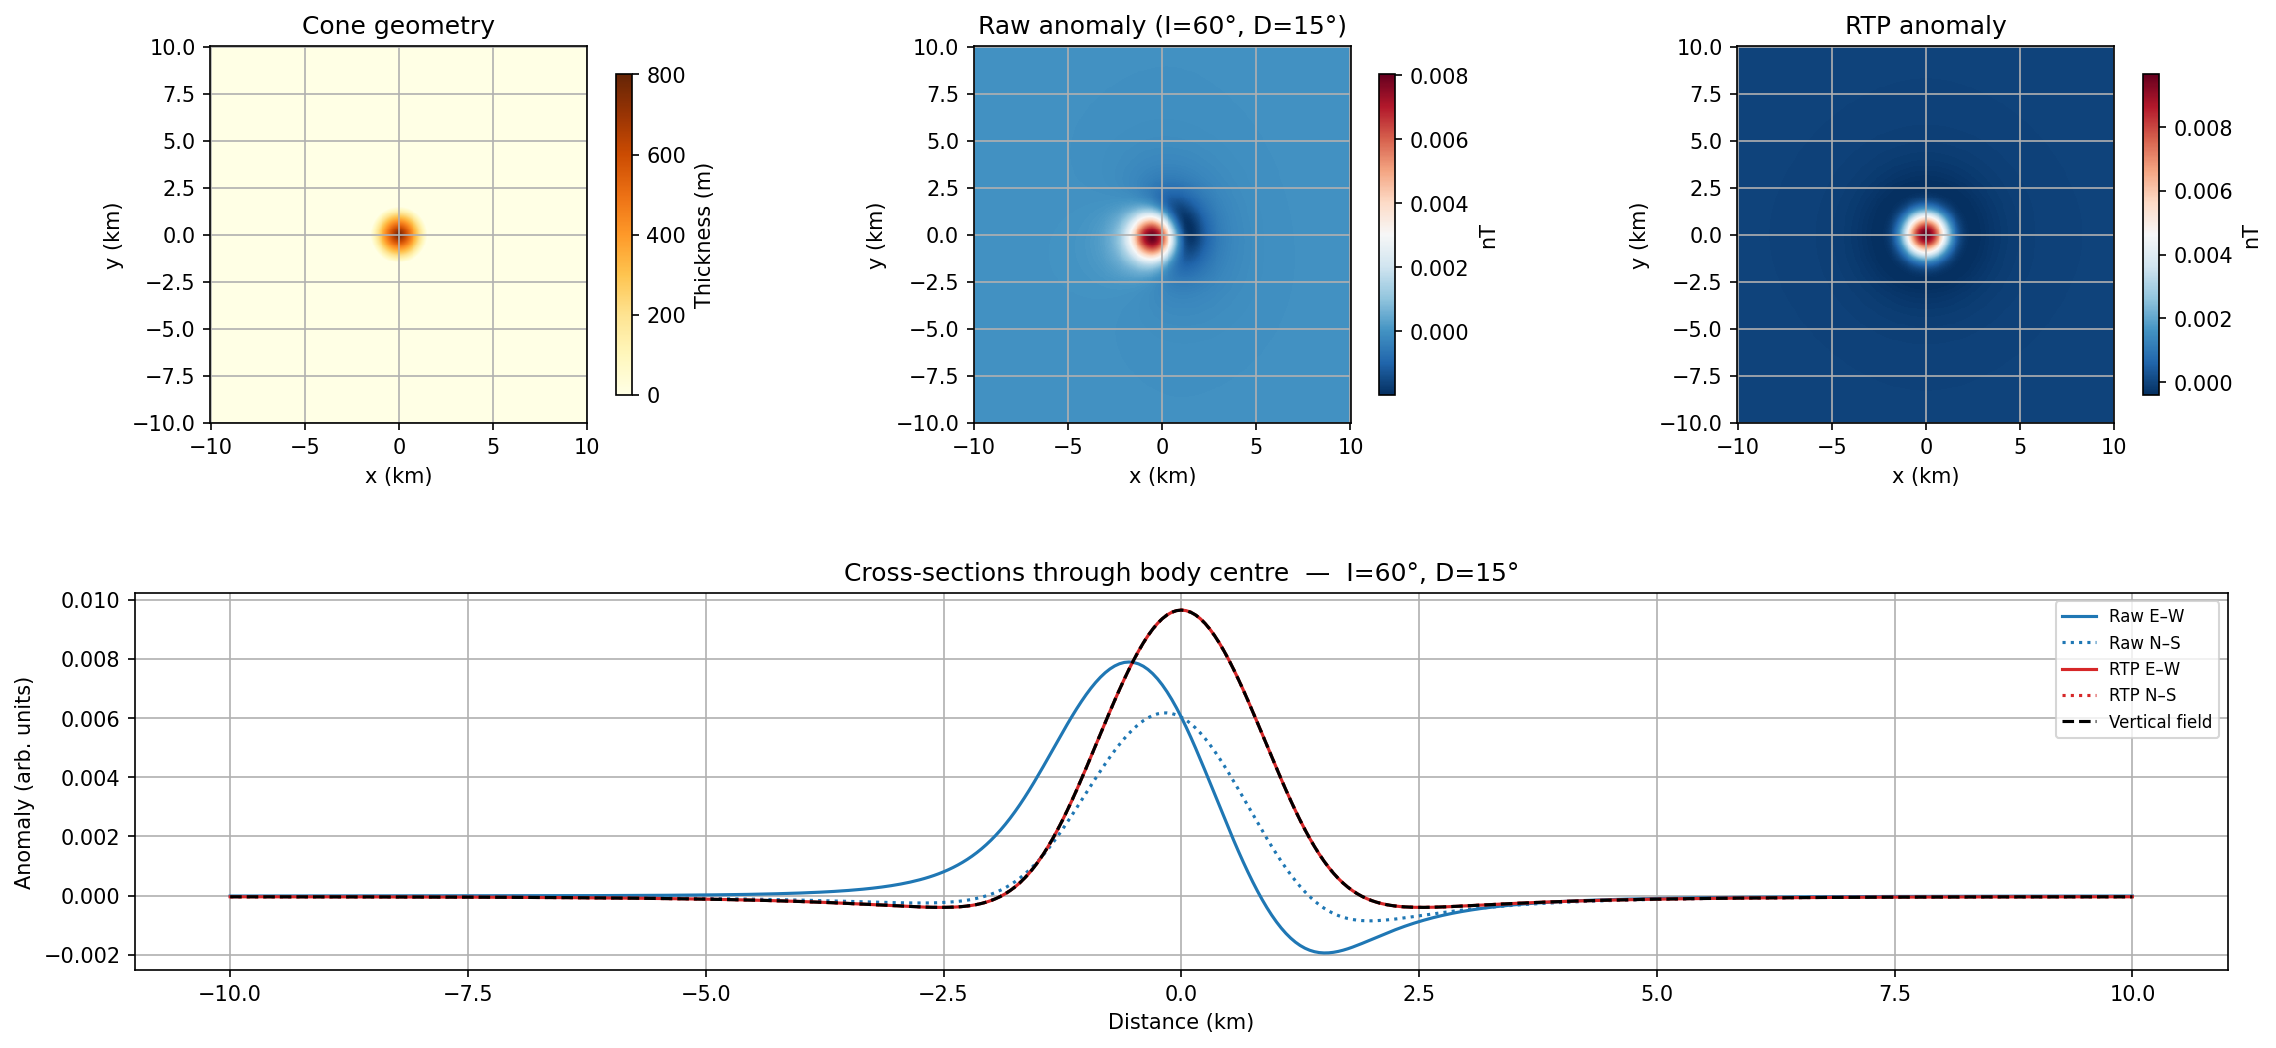
\includegraphics[width=\textwidth]{figures/rtp_pole_reduction.pdf}
            \caption{Cone geometry, raw anomaly, and RTP anomaly (top row) with E--W and N--S cross-sections through the body centre (bottom).}
            \label{fig:rtp_synthetic_result}
        \end{figure}

        \begin{enumerate}[label=\roman*]
            \item Is the RTP anomaly in Figure~\ref{fig:rtp_synthetic_result} more symmetric than the raw one? Is its maximum now centred over the source?
            \answerbox[2cm]

            \item What changed between the raw and RTP profiles -- amplitude, phase, or both? Point to specific evidence in the cross-sections.
            \answerbox[2.5cm]

            \item Using $\Delta y \approx z\cot|I|$ with the cone's burial depth and $I=60^\circ$, estimate the expected shift and compare it to what you measure off the raw-anomaly profile.
            \answerbox[2.5cm]
        \end{enumerate}

    \question{Tower Hill: Applying RTP to Real Data}

        The Tower Hill dataset is an IGRF-corrected aeromagnetic grid ($\sim$10.4\,km $\times$ 13.2\,km, 241$\times$241 pixels, $\sim$50\,m spacing -- far finer than the maar diameter, so aliasing is not a concern here). At the site, $I\approx-70^\circ$, $D\approx+10.5^\circ$, $F\approx60\,000$\,nT. Both the ambient field and the assumed magnetisation direction are set to these IGRF values -- the standard assumption of purely induced magnetisation.

        \begin{figure}[h]
            \centering
            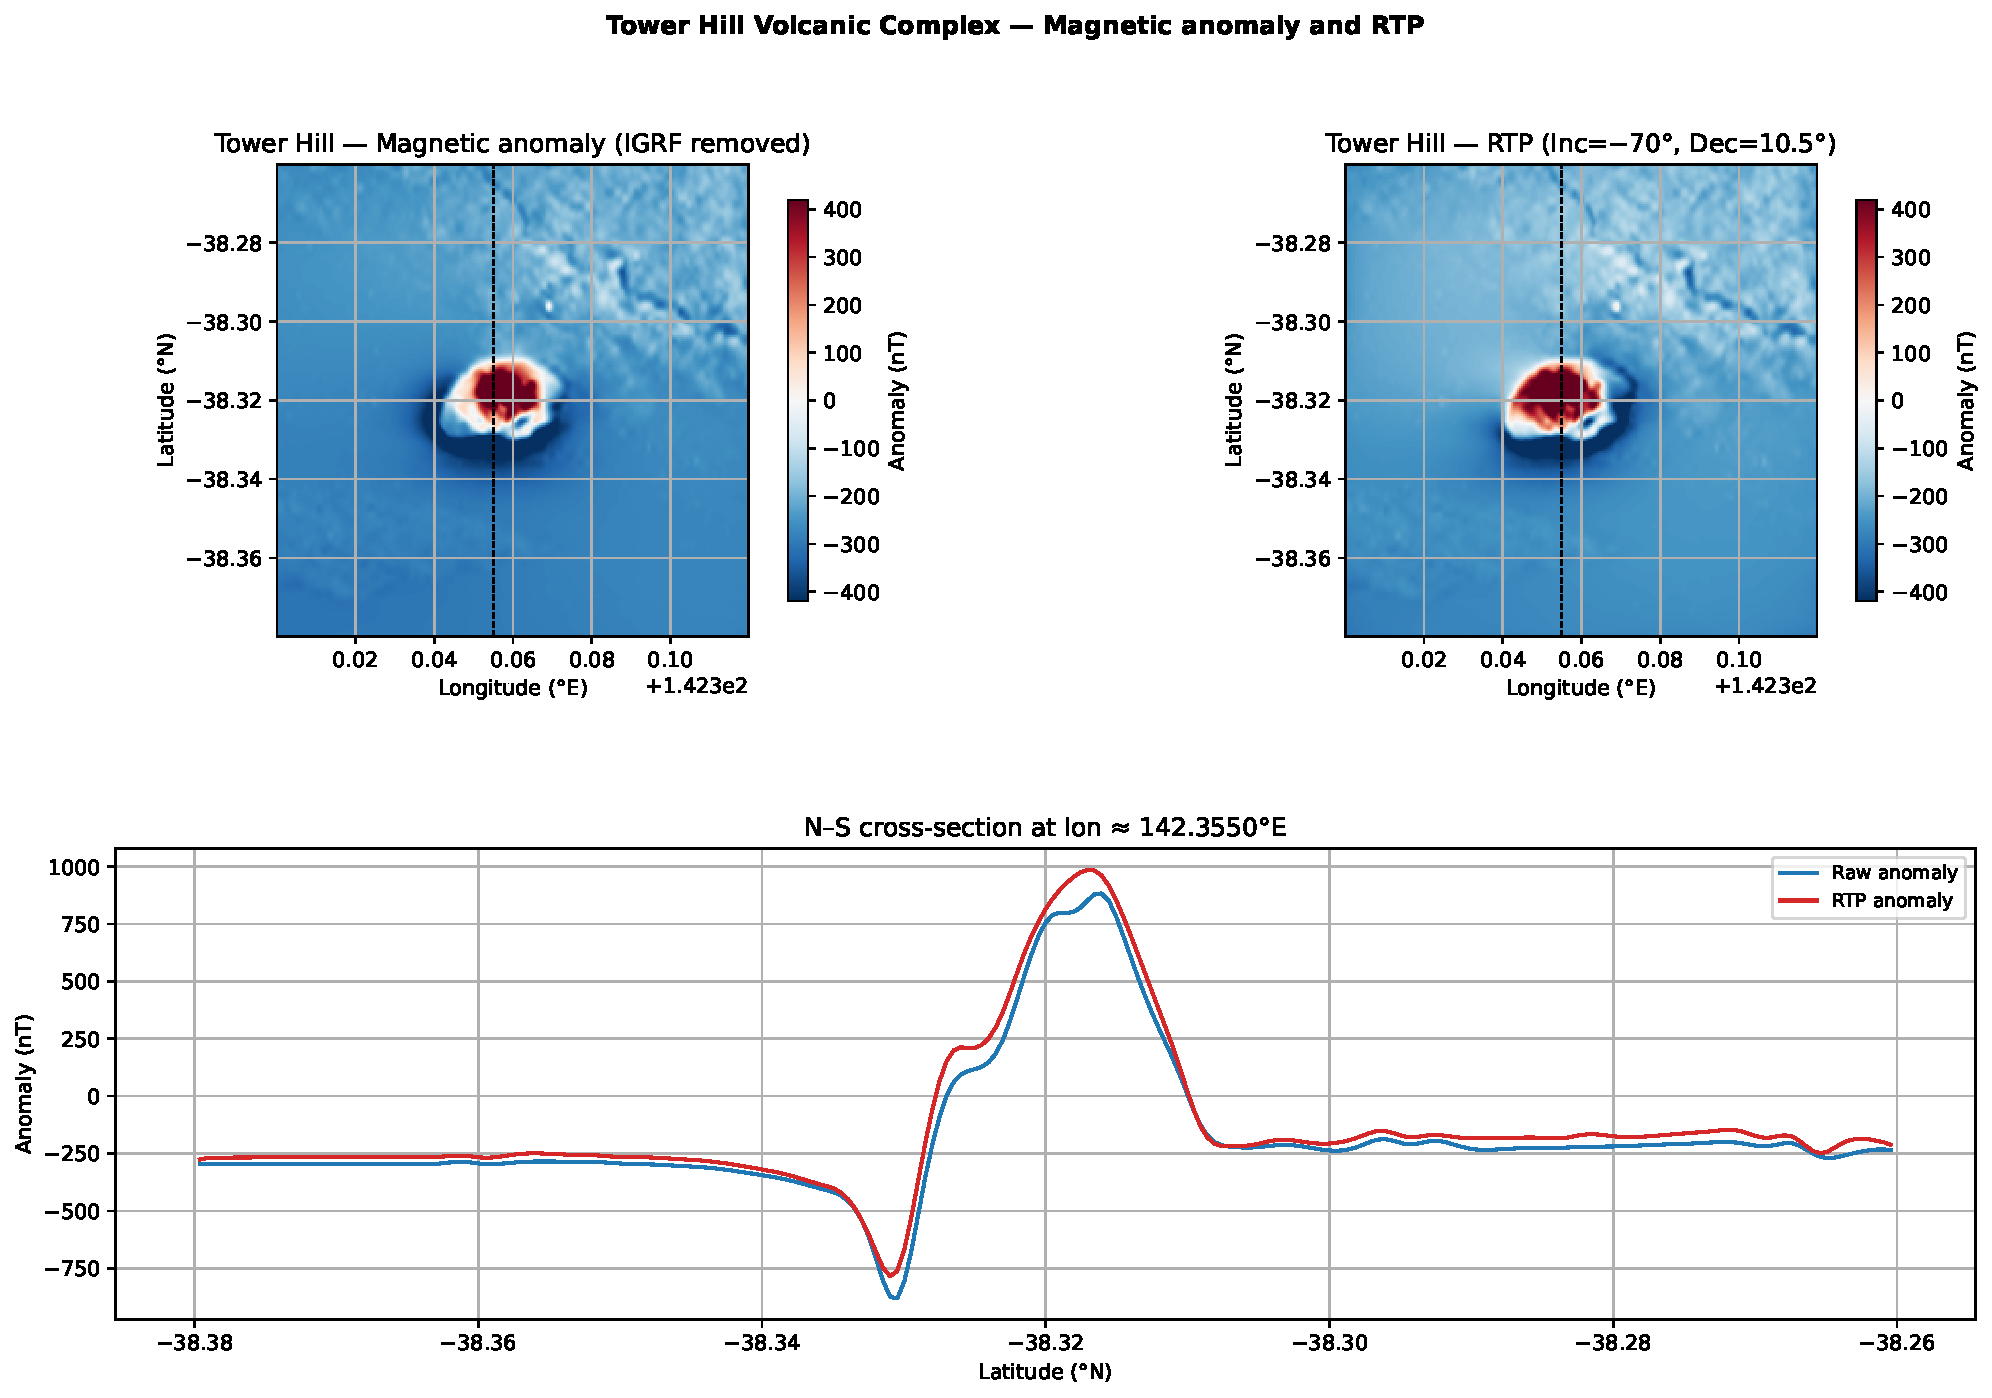
\includegraphics[width=\textwidth]{figures/rtp_tower_hill_real_data.pdf}
            \caption{Tower Hill TMI anomaly (top left), RTP anomaly (top right), and N--S cross-section through the anomaly (bottom).}
            \label{fig:rtp_towerhill}
        \end{figure}

        \begin{enumerate}[label=\roman*]
            \item At $I\approx-70^\circ$ (Southern Hemisphere), which side of the maar centre do you expect the raw positive lobe to sit on -- and does the real data confirm it?
            \answerbox[2.5cm]

            \item Compare the raw and RTP maps. Has the negative lobe south of the peak been reduced, eliminated, or does it persist? What would persistence suggest about the assumption of purely induced magnetisation?
            \answerbox[2.5cm]

            \item The real diatreme's top is estimated at 200--400\,m depth. Using $\Delta y \approx z\cot|I|$ with $I=70^\circ$, does the predicted shift range match the displacement you can measure in Figure~\ref{fig:rtp_towerhill}?
            \answerbox[2.5cm]
        \end{enumerate}

    \question{When RTP Breaks Down: Instability and Limitations}

        The direction-cosine factor $\Upsilon$ approaches zero for wavenumber components aligned with the horizontal field direction as $I\to0^\circ$. Even with water-level stabilisation, the filter then amplifies those components strongly, producing ringing artefacts and unreliable phase corrections. The figure below reruns the exact same pipeline as Question 4, at the same declination, but at $I=8^\circ$ -- well below the stability threshold.

        \begin{figure}[h]
            \centering
            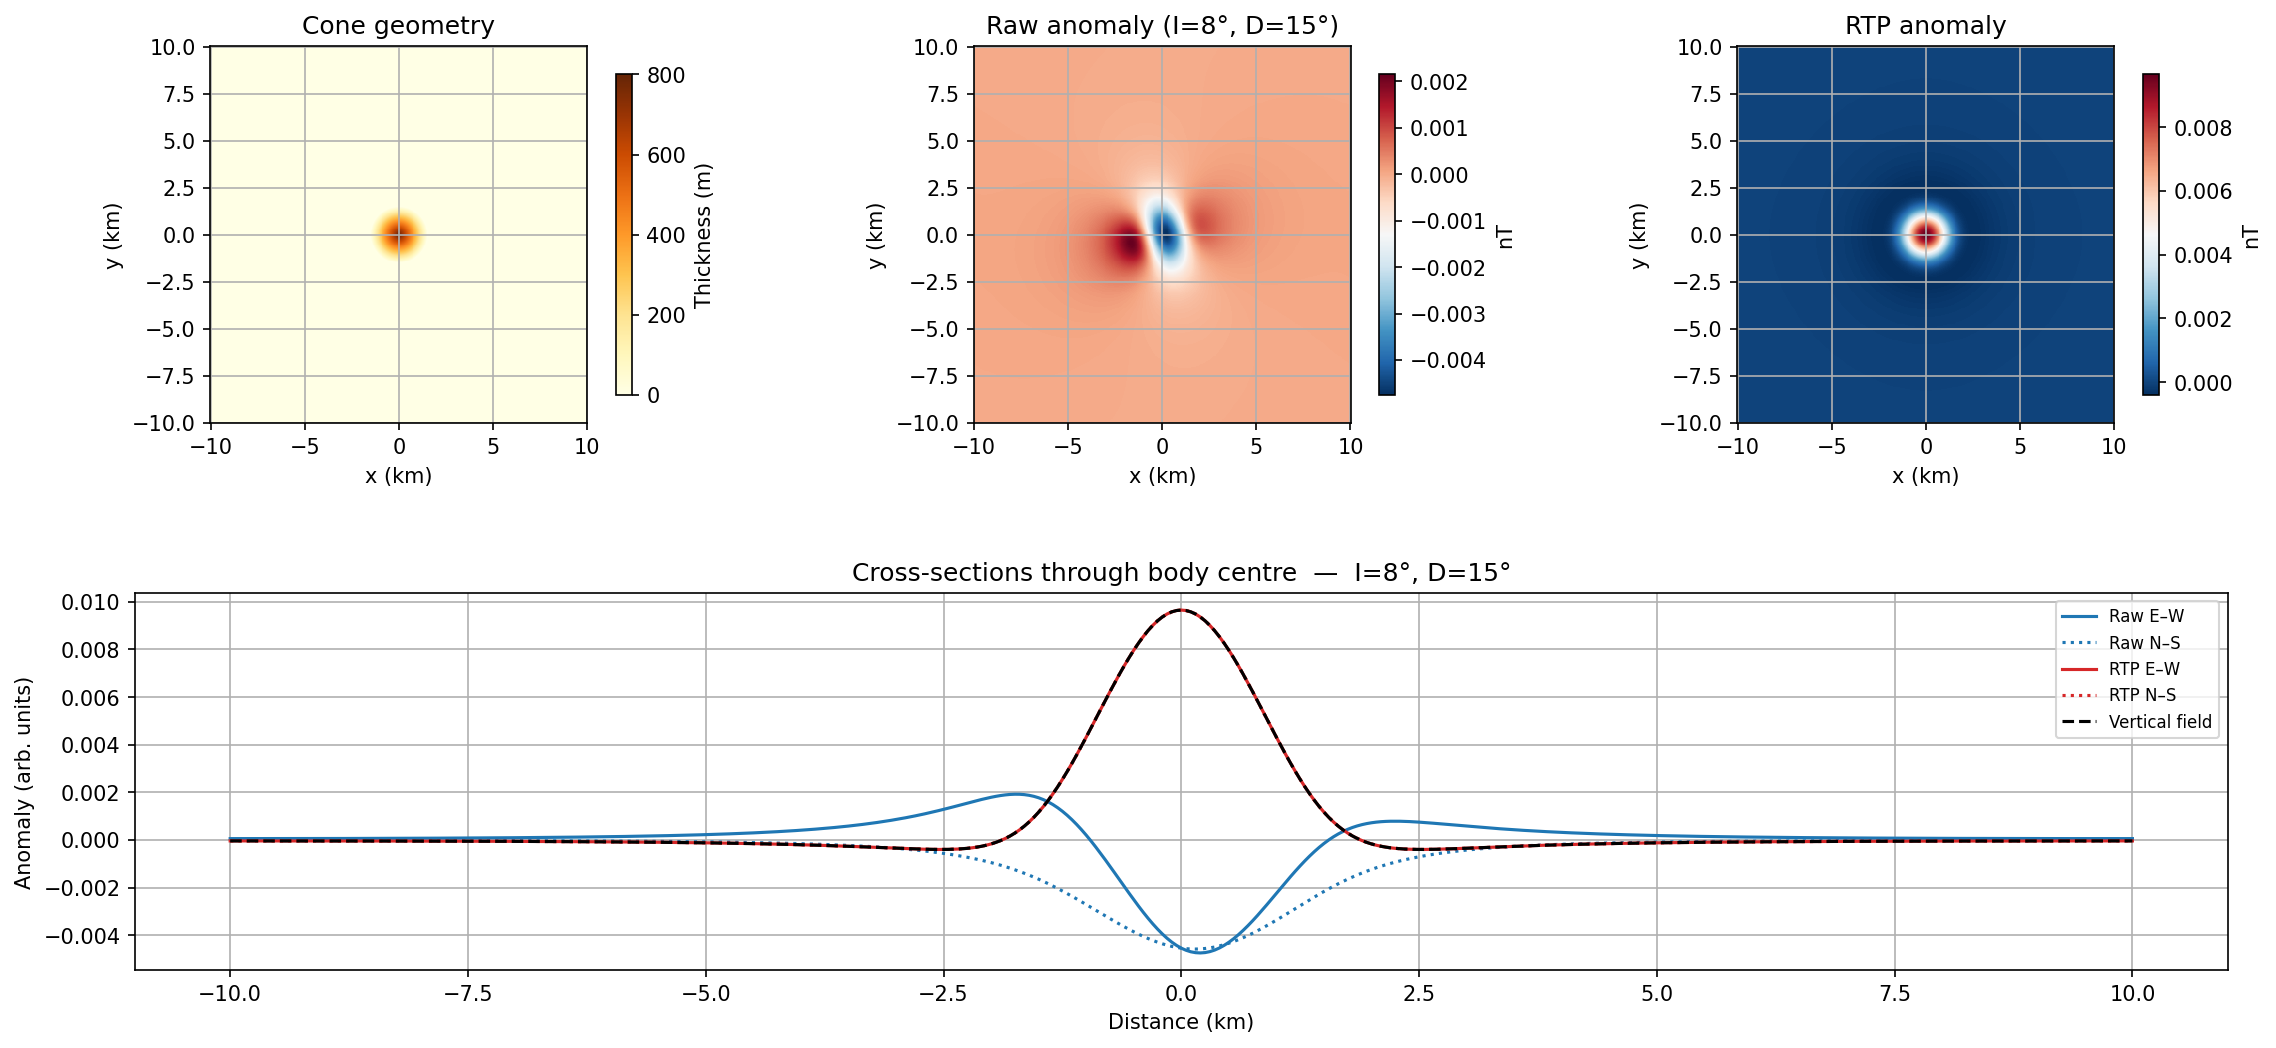
\includegraphics[width=\textwidth]{figures/rtp_low_inclination_instability.pdf}
            \caption{The same forward-model-then-RTP pipeline as Figure~\ref{fig:rtp_synthetic_result}, run at $I=8^\circ$ instead of $I=60^\circ$.}
            \label{fig:rtp_instability}
        \end{figure}

        Beyond low-inclination instability, two further limitations apply specifically to Tower Hill:
        \begin{itemize}
            \item \textbf{Remanent magnetisation.} Standard RTP assumes induced magnetisation parallel to the present-day field. If a rock's frozen-in remanent direction differs from the current field -- common in Quaternary volcanics that experienced geomagnetic excursions -- RTP will fail to centre the anomaly correctly and can produce a \emph{worse}-looking result than the raw data.
            \item \textbf{Heterogeneous magnetisation.} The diatreme fill is a breccia -- a chaotic mixture of country rock, basalt clasts, and matrix -- so the effective susceptibility and remanence vary laterally and vertically in ways a single RTP filter cannot capture. The correction is a spatially averaged one, valid only in bulk.
        \end{itemize}

        \begin{enumerate}[label=\roman*]
            \item Compare Figure~\ref{fig:rtp_instability} to the $I=60^\circ$ result in Figure~\ref{fig:rtp_synthetic_result}. Describe what "breaking down" actually looks like here -- is it a subtle degradation or an obvious one?
            \answerbox[2.5cm]

            \item At Tower Hill's actual inclination ($I\approx-70^\circ$), is RTP operating anywhere near this instability regime? How far (in degrees) is Tower Hill from the threshold you'd estimate from Figure~\ref{fig:rtp_instability}?
            \answerbox[2cm]

            \item Suppose part of the Tower Hill diatreme carries strong remanent magnetisation in a different direction from the present field. Would you expect the standard RTP (which assumes induced-only, present-field-parallel magnetisation) to \emph{under}-correct, \emph{over}-correct, or fail in a way that's hard to characterize as either? Explain your reasoning.
            \answerbox[2.5cm]
        \end{enumerate}

\end{questions}

\section*{Key Ideas}
\begin{itemize}
  \item Magnetic anomalies are asymmetric away from the pole because the direction-cosine factor $\Upsilon(\mathbf{k})$ is complex and direction-dependent; at the pole it collapses to a real constant and the asymmetry vanishes.
  \item RTP is a Fourier-domain \emph{phase} correction: amplitude spectra before and after are nearly identical, while the phase correction varies strongly with direction in $\mathbf{k}$-space.
  \item RTP is stable and reliable at steep inclinations like Tower Hill's ($I\approx-70^\circ$) but becomes singular as $I\to0^\circ$, amplifying noise into ringing artefacts.
  \item RTP assumes induced-only magnetisation parallel to the present field; remanent magnetisation or heterogeneous susceptibility can degrade or invalidate the correction even when inclination itself is not the problem.
\end{itemize}

\end{activity}
